\section{Lógica Nebulosa}

Sistemas nebulosos aproximam funções. Eles são aproximadores universais se usarem regras suficientes. 
Neste sentido sistemas difusos podem modelar qualquer função ou sistema contínuos. Aqueles sistemas 
podem vir tanto da física quanto da sociologia, bem como da teoria do controle ou do 
processamento de sinais. Uma arquiterura funcional generica de um Sistema Nebuloso proposta por
\cite{passos2005datamining} é apresentada na figura \ref{arq_fuzzy}.

A qualidade da aproximação difusa depende da qualidade das regras. Na prática especialistas sugerem regras
difusas ou aprendem-nas através de esquemas neurais através de dados e ajustam as regras com novos dados.
Os resultados sempre aproximam alguma função não linear desconhecida que pode mudar com o tempo. Regras e redes neurais mais apropriadas ao domínio do problema resultam em melhores aproximações \cite{kosko1997fuzzy}.

\begin{figure}
  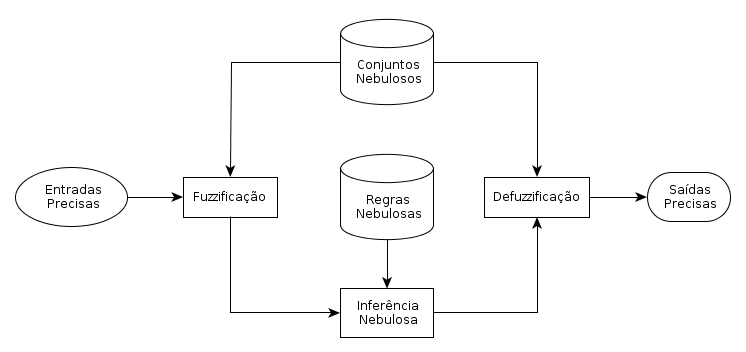
\includegraphics[width=15cm]{imgs/arquitetura_fuzzy}\label{arq_fuzzy}
  \caption{Arquitetura funcional genérica de um Sistema Nebuloso \cite{passos2005datamining}}
\end{figure}

\subsection{Modelo Aditivo Padrão (SAM)}

O sistema difuso $F:\Re^n \rightarrow \Re^p$ é em si uma árvore de regras rasa e extensa. É um aproximador
por antecipação. Existem $m$ regras da forma "Se $X$ é conjunto difuso $A$ então $Y$ é conjunto difuso $B$".
A relação de pertinência "$X$ é conjunto difuso $A$" é descrita por uma função de pertinência
$\mu_A: x \longrightarrow [0,1]$. No diagrama da figura~\ref{arq_fuzzy} esse processo é representado pela
caixa \emph{Fuzzificação}. A regra nebulosa "Se <\textit{antecedente nebuloso}> então <\textit{consequente nebuloso}>" dispara
o processo de \emph{Defuzzificação} descrito no <\textit{consequente nebuloso}>. Esse processo de conecção é conhecido como
\emph{Inferência Nebulosa}.

Cada entrada $x$ aciona parcialmente todas as regras em paralelo. Então o sistema age como um processador 
associativo a medida que calcula a saída $F(x)$.

Essas regras relacionam os conjuntos $A_j$ e $B_j$, gerando o caminho difuso $A_j \otimes B_j$. Na prática,
é utilizado o produto para definir $ a_j \otimes b_j (x,y) = a_j(x).b_j(y)$. Esta é a parte "padrão" no SAM\@.
A parte "aditiva" se refere ao fato de a entrada $x$ acionar a $j$-ésima regra em um grau $a_j(x)$ e o sistema 
soma os acionamentos ou partes escaladas dos conjuntos escalados $a_j(x)B_j$, \cite{kosko1997fuzzy}:

\begin{eqnarray}
F(x) = \frac{\sum w_i.a_i(x).V_i.c_i}{\sum w_j.a_j(x).V_j}
\end{eqnarray}

Com o volume/área $V_j$ e o centroide $c_j$ são dados por:

\begin{eqnarray}
V_j = \int{b_j(y_1,\cdots,y_p)}_{\Re^{p}}.dy_1\dots dy_p > 0\\
c_j = \frac{\int{y.b_j(y_1,\cdots,y_p)}_{\Re^{p}}.dy_1\dots dy_p}{V_j}
\end{eqnarray}

\subsection{Exemplo de Aplicação}

Este exemplo foi retirado de \cite{passos2005datamining}. Deseja-se neste
exemplo determinar qual o valor da apólice de seguro a ser pago pelo
cliente João a partir dos valores de idade e de pressão arterial deste cliente.
Considerando-se as Regras Nebulosas
\begin{itemize}
  \item \emph{SE} idade é \textit{meia-idade} \emph{E} pressão é \textit{baixa} \emph{ENTÂO} seguro é \textit{baixo}
  \item \emph{SE} idade é \textit{jovem} \emph{E} pressão é \textit{alta} \emph{ENTÂO} seguro é \textit{alto}
\end{itemize}

Considere que João tem 35 anos e pressão $(130,70)$. Suponha que as funções de pertinência dão como resultado:
\begin{description}
  \item $\mu_{meia-idade} (35) = 0.8$
  \item $\mu_{jovem} (35) = 0.6$
  \item $\mu_{Alta}(130,70) = 0.5$
  \item $\mu_{Baixa}(130,70) = 0.6$
\end{description}

Logo, para a regras 1 e 2, considerando-se o modelo de Mandani descrito em \cite{passos2005datamining}, tem-se que 
\begin{description}
  \item $0.8$ \emph{E} $0.6 = Min \lbrace 0.8,0.6 \rbrace = 0.6 = \mu_{baixo}(X)$ 
  \item $0.6$ \emph{E} $0.5 = Min \lbrace 0.6,0.5 \rbrace = 0.5 = \mu_{alto}(Y)$
\end{description}

A partir de um processo de defuzzificação, das as distribuições $\mu_{baixo}$
e $\mu_{alto}$, tem-se que:

\begin{description}
  \item $X = 800$ e $Y=700$
  \item $Seguro = \frac{(0.5 \times 800)+(0.6 \times 700)}{0.5 + 0.6} = 745.45$
\end{description}

Assim a apólice de seguro a ser paga por João será de $745.45$ reais.

\subsection{Aplicação ao problema}

Para aplicar esse método ao problema analisado neste trabalho é necessário definir as regras e as distribuições
das variáveis.

A vantagem dos conjuntos difusos é que eles tornam o modelo mais robusto. A lógica fuzzy
tentam melhorar a classificação e os sistemas de decisão 

A principal desvantagem deste método a modelagem necessária para encaixar os conceitos descritos acima.
Isso, pois o conceito de conjuntos nebulosos ainda estão em desenvolvimento para o problema abordado
neste trabalho. Essa modelagem não é imediata, pois o problema é de classificação temporal. Não basta que
as características do ambiente sejam associadas a conjuntos nebulosos de características. É necessário
que regras sejam especificadas estática ou dinamicamente. No caso estático, elas seriam incorporadas
ao modelo através de especialistas. No caso dinâmico, uma solução é utilizar um classificador para
deduzir as regras.
